\section{Targeted pre-2025 training extension}
The earlier models remain unvalidated. This separate experiment targeted CGAU P/S,
CLAC S, CREM P/S, CSOC P/S, CRUS P/S and CUMA P/S without using 2025 observations
for waveform review, association, fitting or model selection. All prior velocity
trial files remain unchanged. The previously examined 62-event, 1,065-arrival
2025 set was hash-locked and evaluated only after all 18 training fits were frozen.
It remains a reused validation set, not a newly collected blind test.

\paragraph{Coverage and arrival review.}
The missing training support principally reflects different station epochs:
the previous qualifying training events end in May 2024, whereas EIDA advertises
these stations from July--November 2024. The six target stations were retrieved
for 12 and 19 December 2024, 00:00--06:00 UTC, after availability checks.
All 12 requests succeeded: 123,535,872 bytes and 216 core channel-hours.
The measured-size estimate was 123,116,584 bytes. The existing 40 GiB free-space
reserve plus 8 GiB processing allowance remained intact; the broad queue was stopped.
An additional seven event-selected station clips (615,936 bytes) provide network
ties, not continuous detection or completeness exposure.
No requested-but-absent duration is counted as coverage.

The continuous batches yield 1,205 P and 6,132 S picks. Their three initial associations are provisional.
Review of raw and filtered traces identifies a December 12 packet that was split
by later coda picks. A clear raw CGAU P onset was measured at 04:34:26.21 UTC
(reading uncertainty approximately 0.03 s); the earlier existing CRUS S pick
at 04:34:27.44 UTC replaces the later 28.31 s coda pick. These are Codex visual
measurements, not human-reviewed ground truth. Ambiguous CUMA and CSOC phases
remain excluded. The reviewed reassociation has 10 P, 10 S and a 156.2-degree
gap, passing the unchanged pre-inversion screen. Its provisional starting depth
changes from 3.28 to 2.84 km after review; neither value establishes true depth.
The December 19 candidate fails P/S causality and the existing event screen.

The training set increases from 52 events/827 arrivals to 53/847; the selection
sensitivity uses 63 events/1,010 arrivals. Seven previously absent target
station/phase pairs gain one observation each. CSOC P/S and CUMA P/S still have
none. A single event does not independently constrain station corrections across
dates and source depths. All inspected new headers match their StationXML epochs,
responses, rates and coordinates; absolute clock accuracy has not been independently verified.
The 827 inherited training arrivals are preserved, not all newly reviewed.
Earlier uncertain picks and coda associations in that set remain a possible
contributor to instability; this extension does not establish their validity.

\paragraph{Frozen-model validation.}
The same three parameterizations and six sensitivity choices were retained:
$\pm5\%$ initial velocities, training selection, tenfold velocity damping,
32/64-bit fitting and additional iterations. P/S weights remain 1/0.5.
Both fitted families and the zero-delay restricted alternative are reported;
none is selected by its 2025 score. Fixed-model evaluation adjusts held-out
origin times and locations, so this is conditional arrival prediction, not
validation against known hypocenters. The acceptance limits remain 100 m
horizontal displacement, 0.1 km depth, 0.05 km/s velocity and 0.02 s station
delay, together with physical velocities, convergence and improved holdout RMS.

\begin{center}\small\begin{tabular}{lccc}\toprule
Parameterization & Training RMS (s) & 2025 RMS (s) & All gates\\\midrule
Four layers, damped delays & 0.2171 $\to$ 0.1750 & 0.2406 $\to$ 0.2458 & Fail \\
Three layers, damped delays & 0.2174 $\to$ 0.1784 & 0.2432 $\to$ 0.2463 & Fail \\
Three layers, zero delays & 0.2174 $\to$ 0.2115 & 0.2432 $\to$ 0.2272 & Fail \\
\bottomrule\end{tabular}\end{center}
None passes every gate. Across the registered sensitivities, maximum depth
changes are 1.18, 1.39 and 1.57 km for the three families in table order.
The zero-delay family's maximum horizontal change is 898 m and velocity
change is 0.27 km/s. Extra training iterations still change locations by
177 m horizontally and 0.15 km in depth. Its 32/64-bit printed results agree,
but that agreement does not resolve starting-profile and event-selection sensitivity.
After the training decisions were frozen, 1,043 of the 1,065 holdout arrivals
have a represented station/phase combination and 22 remain unrepresented.
Both fitted-delay families worsen RMS even on the represented combinations;
the remaining four empty training cells cannot alone explain the failure.
Independent sums of layerwise ray travel times, with station delays, agree with
the serialized residual calculation to 0.0040--0.0057 s RMS, consistent with
rounded native outputs. This checks arithmetic consistency, not phase truth.
\begin{figure}[H]\centering
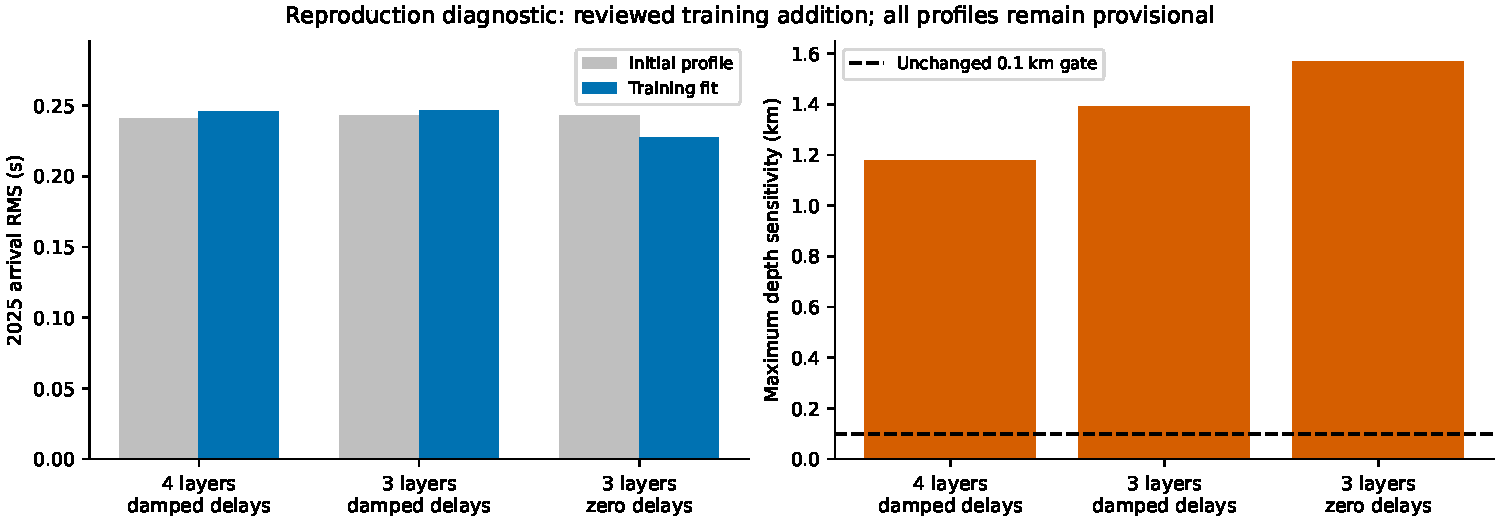
\includegraphics[width=.96\linewidth]{data/velocity_holdout_review/training_extension_20261015/validation_diagnostic.pdf}
\caption{Reproduction diagnostic, not a manuscript panel. Conditional arrival RMS
and maximum depth changes across the registered starting-profile, selection,
damping and arithmetic tests. Saved fits supply all plotted values.}
\end{figure}

\paragraph{Depth coverage and remaining limitation.}
The preserved three-layer zero-delay fit had 80/366 P and 115/461 S paths
in the layer beginning at 3 km. That count includes interface paths: only
48 P and 76 S rays, from nine source events, extended strictly below 3 km.
The numerical ray vertices have 0.01 km precision; these are model-dependent
paths, not measured depths. The new event's fitted depth ranges across trials from
2.70 to 3.04 km.
The addition therefore does not by itself establish improved deep resolution.
In the new zero-delay base fit, 52/376 P and 83/471 S paths extend strictly
below 3 km, but none of those strict deep paths belongs to the added event.
The count change reflects changes to the estimated geometry of older events.
Detailed layer lengths, depth coverage and per-station residuals are saved beside
the fits. More clear pre-2025 events recorded jointly at the target and established
stations, especially with stable depth constraints, are needed. The CSOC and CUMA
records in these two batches do not supply reliable training arrivals. Additional
public pre-2025 intervals remain available but were not downloaded in this bounded
experiment; this is insufficient reviewed coverage, not a claim of inaccessible data.

\paragraph{Reproducibility and status.}
The versioned record is \path{data/velocity_holdout_review/training_extension_20261015/}.
It contains request receipts, coverage and checksums, reviewed arrivals, numerical
fits, residuals, sensitivity results and ray paths. Commands and input placement are
in \path{docs/TARGETED_VELOCITY_TRAINING.md}. The previous empirical panels and
comparison images retain their original checkpoints; no failed profile is promoted
to a calibrated catalog or relocated result.
